\chapter{Experiment design}

This chapter presents the experimental environment used during the development of this work. The first two sections will focus on discussions around the choices of data domain and the CNN architecture. The next section explains all the networks variants, techniques and parameters used during the training process. The two subsequent sections are dedicated to explain the reasons behind the chosen perturbation method and the synthetic generation of the imbalanced dataset, which are the core ideas behind this work.
\section{Data domain}

Our experiments aims to investigate the relationships of the underlying learning structure of CNNs and the perturbation caused by gradient sign methods. In particular we focus on the investigation of how the gradient step from the sign method moves the points away from their distributions, and how this could be affected by both balanced and imbalanced training sets. This requires  class labels of the data set to be non-hierarchical so we can make better assumptions of their distributions. 

We use the CIFAR-10 data set \cite{krizhevsky_2009} in our experiment. CIFAR-10 data is visually rich and empowers the analysis between different class labels. The data set contains 32x32 images in 10 classes, each has 5,000 samples for training and 1,000 for testing. There is not much overlap nor hierarchical relationship between classes. Most CNNs experiments nowadays uses the 2014 ImageNet dataset \cite{deng2009imagenet}. However, its hierarchically organized categories adds unnecessary complexity to the experiment design hindering the analysis of the results (e.g. causality relationships).
\section{The VGG Architecture}

As described in Chapter 2, a CNN is a sequence of layers where every layer transforms one volume of activations to another through a differentiable function. Three main types of layers are used to build these networks: Convolutional Layer, Pooling Layer and Fully-Connected Layer. A Convolutional Layer computes the output of neurons that are connected to local regions in the input, the Pooling layer performs down-sampling operations along the spatial dimensions of the input and, finally, the Fully-connected layer computes the class scores of the classifier. The chosen architecture should have enough layers for learning good features from the training set domain. For instance, a CNN Architecture for CIFAR-10 could have the following configuration: [INPUT - CONV - RELU - POOL - FC].

Network architectures with higher accuracies have better generalization over the overall data input domain, however, adversaries are efficient into extrapolating the given domain by going to previously unseen regions of space (known as domain shift \cite{papernot2016}). For this work we had to make a choice of which network architecture would not only provide reasonable accuracy for our selected data domain (CIFAR-10) but would also be reasonable on the resource consumption. This way we can reproduce the requirements of a real world system where not only accuracy is taken into account when selecting a deep learning model.

From all networks tested on Canziani et al (2016), the VGG16-19 from Simonyan et al. (2014)  seemed to have the best trade off between accuracy and performance (inference time). The VGG architecture won the first and second places on the ILSVRC-2014 submission on the localisation and classification task. The main contribution of the VGG network was to show that the depth of the network is a critical component for good classification performance. The model can be assembled with 16 or 19 Conv/FC layers and it features an extremely homogeneous architecture that only performs 3x3 convolutions and 2x2 pooling from beginning to end.

\begin{figure}[!h]
	\centering
	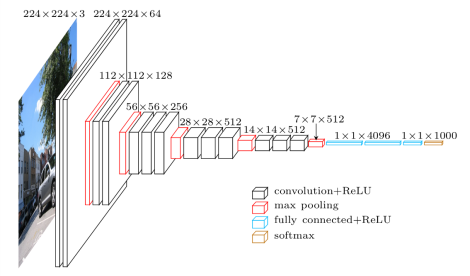
\includegraphics[scale=0.6]{imagenet_vgg16.png}
	\caption{VGG16 on ImageNet}
	\cite{simonyan2014very}
	\label{fig:vgg16}
\end{figure}

The design of the VGG16 has been proven to work even on datasets with several classes that are very different from each other . The two last fully connected layers of the state of the art model are comprised of 4096 neurons each, leading to much higher parameters complexity. As the dataset used in this work has only 10 classes, the two FC-4096 layers were replaced by one single layer with 512 neurons and RELU activations. This helped to reduce over-fitting when training the network. In addition, the total number of convolutions blocks and pooling were reduced to 3, with the first layer having 2 stacked convolution layers followed by a max pooling of stride 2x2 and the last two layers with 3 stacked convolutions also followed by a max pooling of stride 2x2. The max pooling layers are responsible for reducing the image size by 50\% every time an image passes through it. Since CIFAR-10 images are only 32x32, the original VGG16 architecture would end up having an output of shape of only 1x1 pixel at the last layer. In order to avoid this problem, the number of layers were reduced so to fit our dataset domain. The resulting shape fed into the fully connected layers is 4x4x128 (Width x Height x Channels) as it can be seen on table ~\ref{tbl:vgg10}. 

\begin{table}[!h]
	\centering
	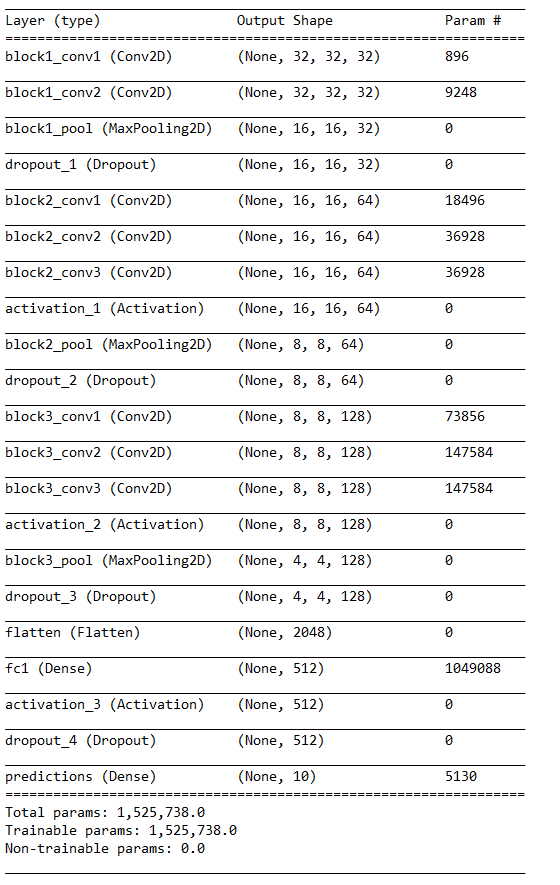
\includegraphics[scale=0.9]{vgg_arch.png}
	\caption{Full Model Description}
	\label{tbl:vgg10}
\end{table}
 
\section{Overall Training Process}

Neural Networks require good optimisation methods in order to achieve good performance. As networks get deeper, the number of resources required to train increases considerably. CNNs can share parameters within its convolution layers, thus, reducing the amount of computation needed during the training stage. All the models in this work were implemented using Python programming language along with Tensorflow and Keras frameworks. The first is a high performance calculation engine that uses GPUs to accelerate its matrix/vector calculations. The latter is a Neural Network library that helps on the implementation of any deep learning model. Keras is mainly a wrapper on top of tensorflow that hides some abstraction from the developer, making it one of the best frameworks for DNNs currently.

As discussed on Chapter 2, the full gradient update would not be the best choice for optimizing deep networks. Stochastic Gradient methods were one of the first methods developed to overcome this problem and are still being further developed nowadays. The SGD based optimisation technique used in this work was developed by Bengio (2015) \cite{bengiormsprop}, namely RMSProp. This method is an adaptive learning rate scheme that can take the absolute values of the Hessian's eigenvalues and, therefore, approximate the equilibration pre-conditioner. As shown on Bengio's work \cite{bengiormsprop}, the method outperforms current SGD methods by achieving convergence faster.The learning rate for the method was set at $10^{-4}$ and the decay $10^{-5}$.

In order to achieve optimal accuracy, every algorithm should be trained until convergence, in other words, it does not under-fit or over-fit the given dataset. Avoiding over-fitting and under-fitting is highly important when training DNNs. Our architecture was trained until no more reasonable changes were detected in the validation loss so we could dismiss unnecessary training steps and consequently any kind of over-fitting. This was achieved by using the Early Stopping technique as described on \cite{stanford2016}. Fundamentally, this consists of a functional callback that runs at the end of every epoch and compares the previous loss with the current one and interrupts training if the difference was below an user provided $\delta$ for a specific number of steps in a row. The value of our $\delta$ was set at $10^{-4}$ and the number of steps to 10. For instance, training would be stopped if no improvement over the specified $\delta$ was seen for 10 steps in a row. Also, we did put a hard limit of 200 on the total number of epochs.

\begin{figure}[!h]
	\centering
	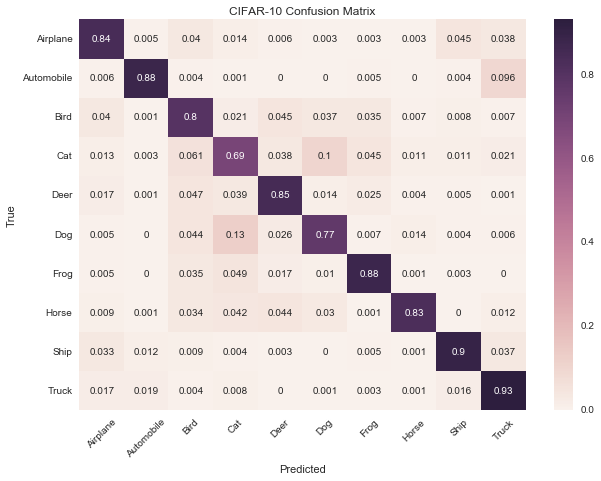
\includegraphics[scale=0.6]{conf_matrix.png}
	\caption{Results on the full dataset}
	\label{fig:conf_matrix_full}
\end{figure}

The confusion matrix helps understanding the individual score for each class and also provides information of the ratio on which the true class was misclassified as other classes. Figure ~\ref{fig:conf_matrix_full} shows that the Cat and Dog classes are often interchangeably misclassified as they have a set of similar features. The network have reached an overall accuracy of 83.45\% and a total validation loss of 0.5033.

\section{Perturbation method}
The gradient sign is a method that uses internal gradient information to create directed perturbation to input data. The resulting label will be different whether one adds or subtracts noise according to equations 1 and 2. 

\begin{equation}
C(x + \delta)\approx C(x) + \epsilon * sign(\nabla C)
\end{equation}
\begin{equation}
C(x + \delta)\approx C(x) - \epsilon * sign(\nabla C)
\end{equation}

The gradient sign equation has a simple interpretation. The main goal is to add a change $\delta$ into each pixel of the image so as to make that image closer to the chosen label on which we extracted the gradient from the source network. The sign on our $\nabla C$ indicates that we are only interested on the direction of the gradient while the $\epsilon$ controls the magnitude of the step.

\begin{figure}
	\centering
	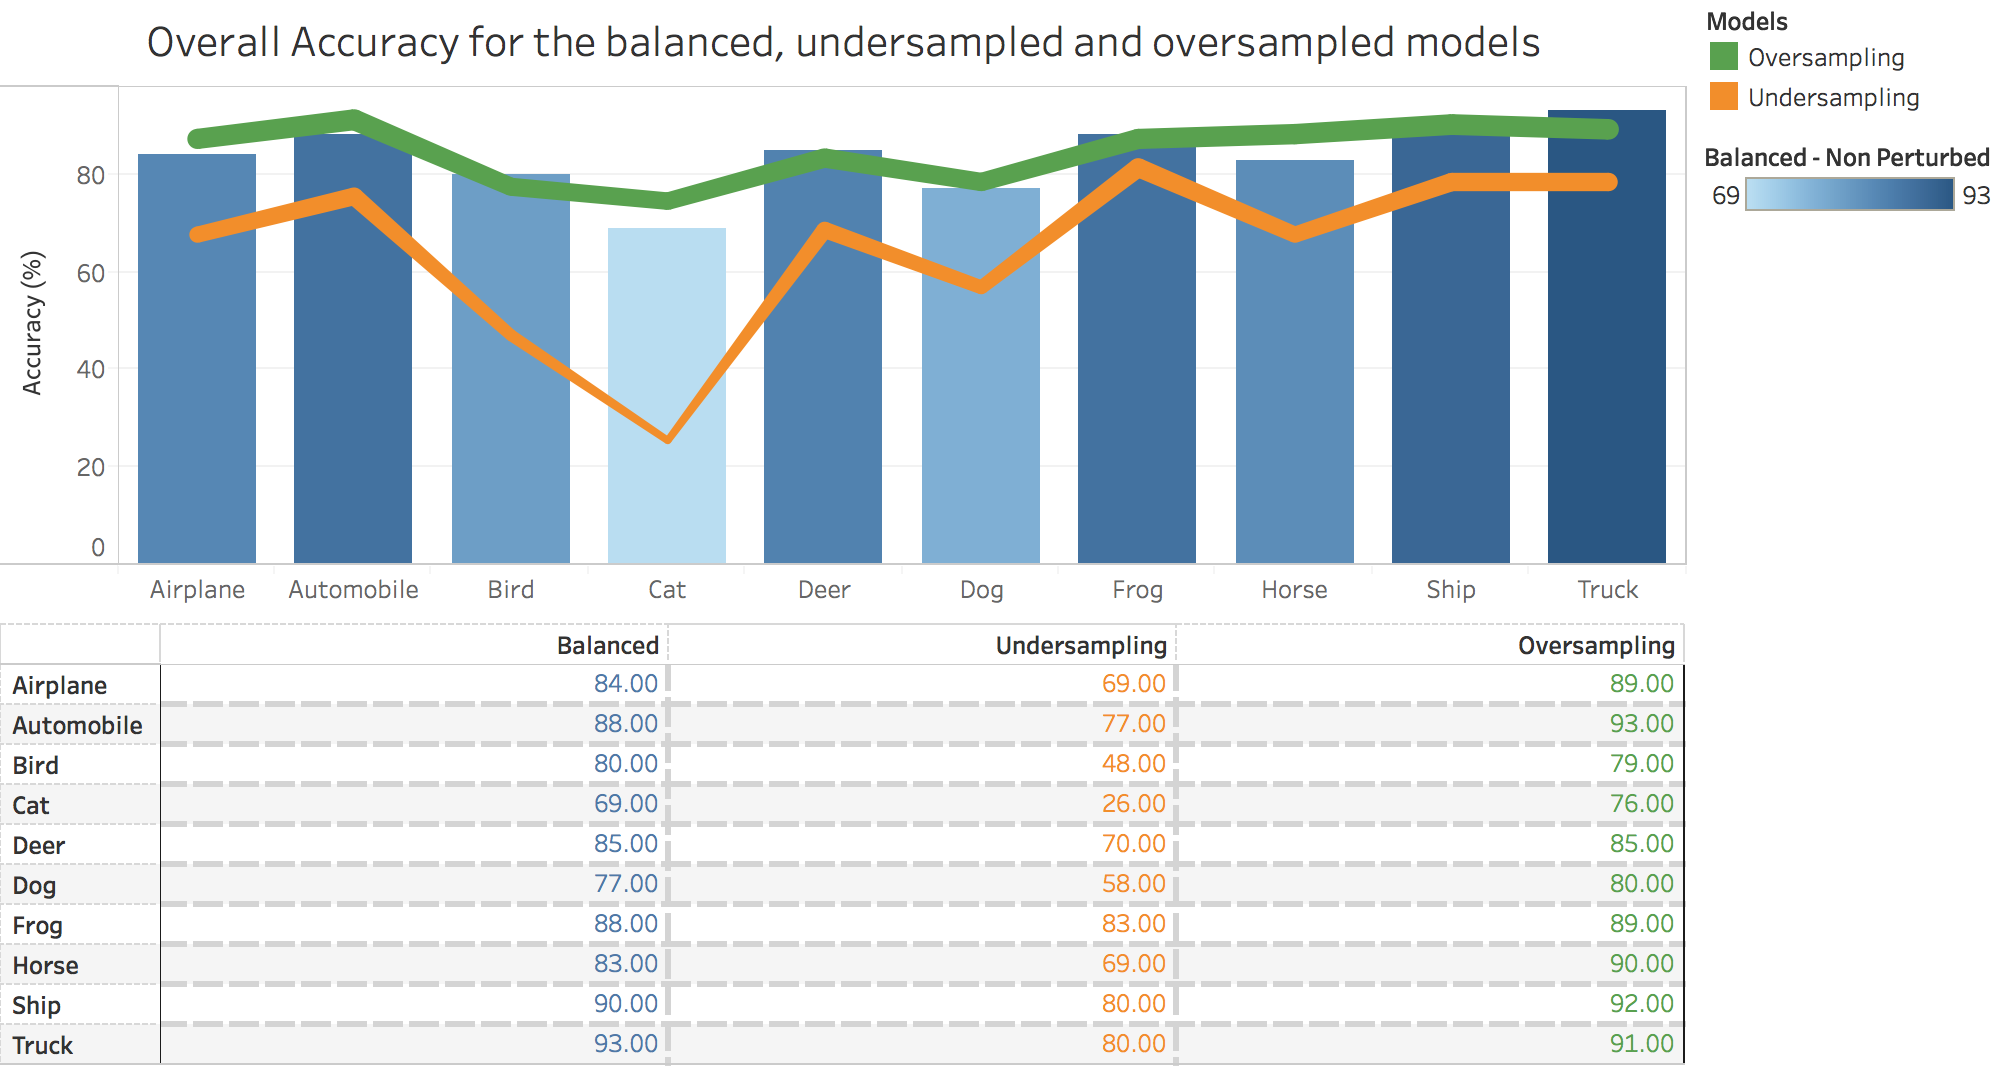
\includegraphics[height=6.5cm]{graph_non_pert.png}
	\caption{Individual class accuracy for under-sampled, over-sampled case on the CIFAR-10 modified dataset shows a decrease in accuracy for classes with lower number of samples}
	\label{fig:acc_graph}
\end{figure}

Suppose the current true label of the class is selected as a gradient candidate, adding noise would mean that we increase the cost function of our input while subtracting noise is the same as minimizing our loss function even further. The equations above are usually referred as ascent and descent methods

Perturbations could also be applied by two variations of the gradient sign method. While the fast gradient sign method applies a single perturbation to the input, the iterative gradient sign method performs the same perturbation a chosen number of times iteratively \cite{goodfellow2014}. 
\section{Synthetic data imbalance}

Classification models are usually required to have similar number of samples for each class in order to equally learn proper feature representations for each label. As shown on Murphey and Guo (2004) \cite{murphey2004}, Neural Networks have lower generalization capabilities and are biased towards specific classes when trained on datasets with unequal number of samples between classes. 

As the CIFAR-10 dataset is not naturally imbalanced, we have artificially created two variations on which we trained the imbalanced networks.  One dataset consists of a direct under-sample of the target class to 1,000 samples, and the other was changed using  an oversampling of the target class (or an under-sampling of all other classes). We kept the number of samples for the target class at 5,000 while all other classes were reduced to 1,000 samples. For each class of the two different datasets configurations, a network was then trained until convergence using the same hyper-parameters as the balanced case. Each model was evaluated against a test set of 1,000 samples of the target class which was  perturbed by its own under/over-sampled model and the balanced model. The two sources of gradient information are referred as white-box and black-box attacks since the former has complete information of the network weights and biases while the latter uses an approximation of the same parameters. 

Both imbalanced networks were separately tested for each class on white-box and black-box adversarial attacks. The white-box test was designed to investigate the vulnerability of class imbalance on adversarial examples while the black-box test is designed to verify the robustness on transfer learning environments. In total we evaluated 50 different combinations: 20 for each different imbalanced dataset (same model gradient and balanced network gradient) and 10 for the balanced network using its own gradients on each class. Figure~\ref{fig:acc_graph} shows the accuracy for the models without any perturbation. It can be seen that the individual class accuracy for the under-sampled case is reduce while the same metric is increased on the over-sampling network. 

\begin{figure}[!h]
	\centering
	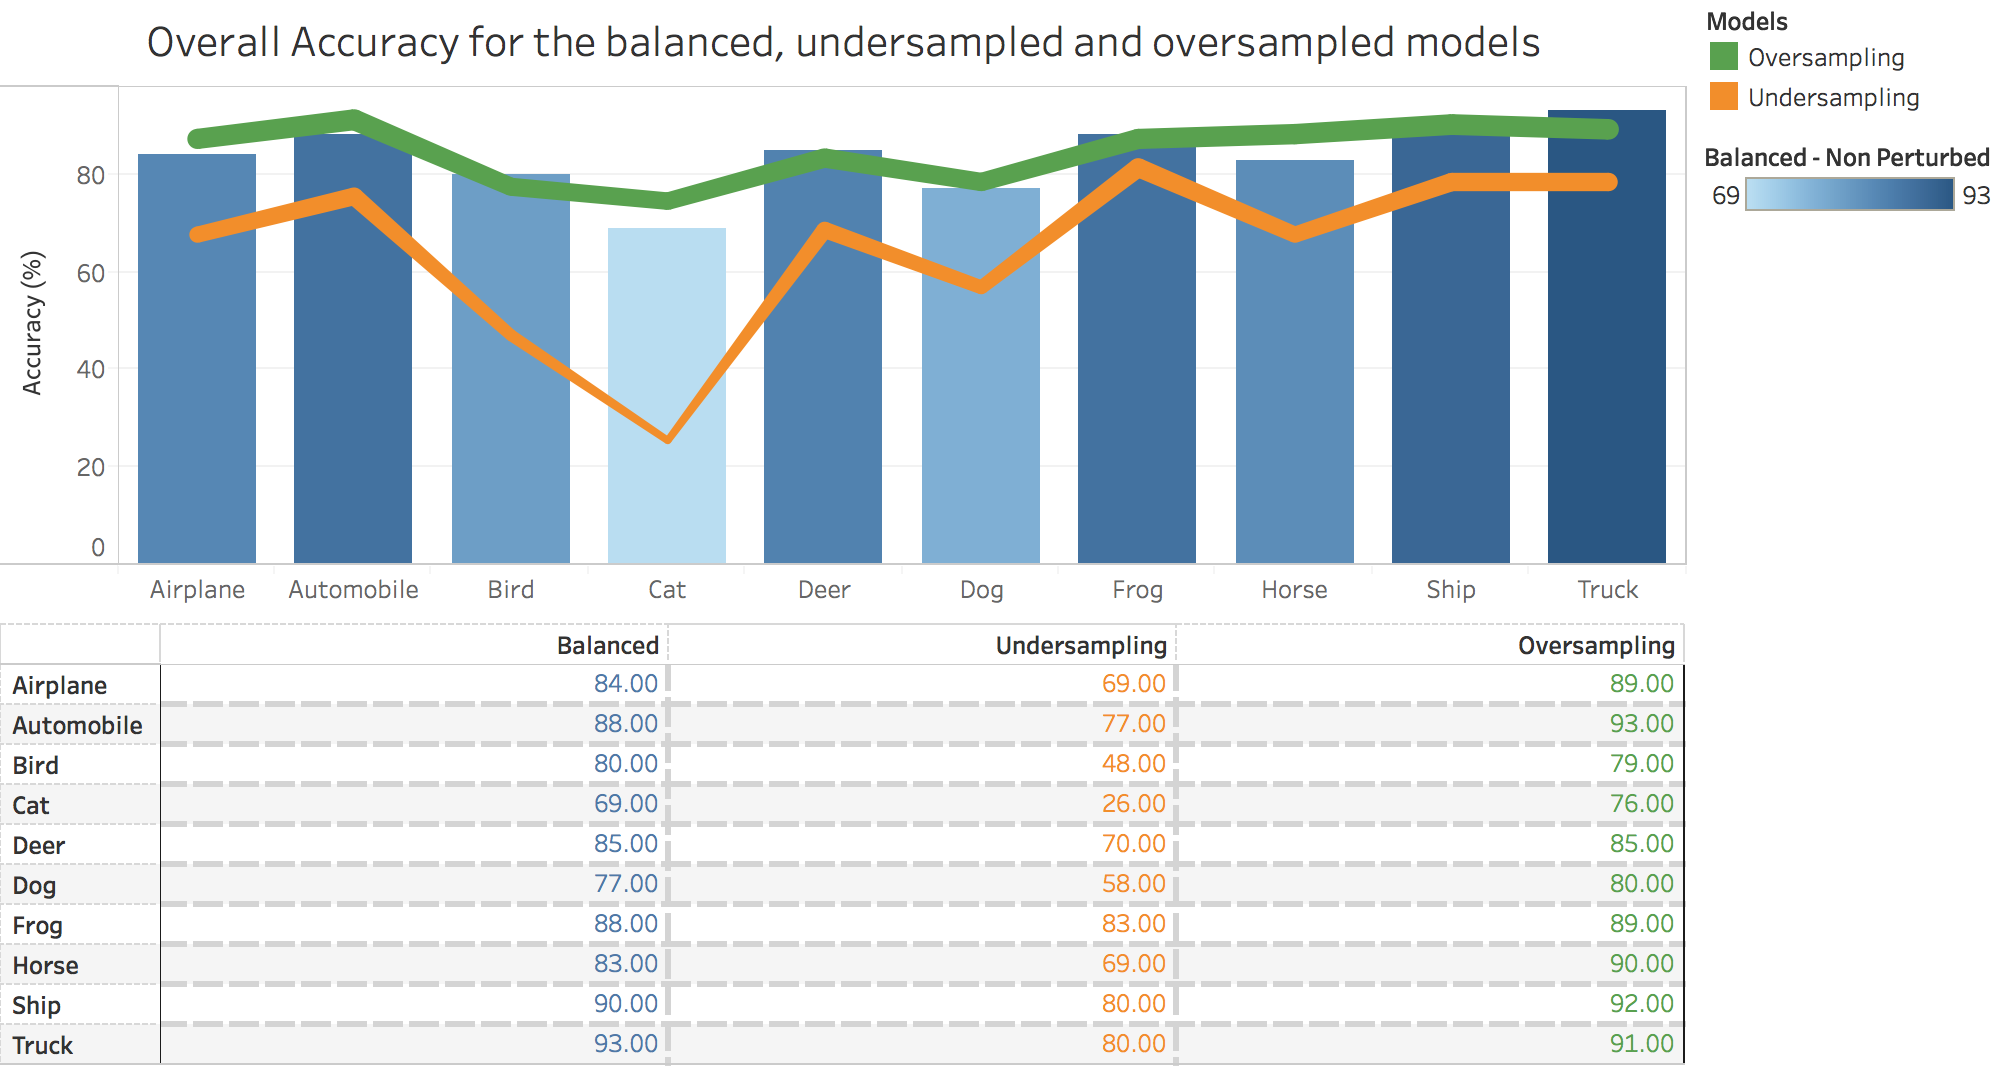
\includegraphics[scale=0.3]{graph_non_pert.png}
	\caption{Target class accuracy on all models}
	\label{fig:acc_graph}
\end{figure}

Figure ~\ref{fig:acc_graph} shows the per class accuracy for each specific model on non-perturbed test set. While the over-sampling on the target class causes the per class accuracy to increase, the down-sampling causes the same accuracy to be drastically reduced when compared to the balanced model shown on figure ~\ref{fig:conf_matrix_full}. The former happens because the model learns more about the target class due to its increased number samples, hence, it concentrates on learning the specifics of the class rather than equally splitting its capacity through all classes as it happens on the latter. The increased accuracy means that the model better explores the space around the target class since it does not have enough evidence to explore other classes spaces.

